% !TeX root = ../main.tex
% Add the above to each chapter to make compiling the PDF easier in some editors.

\chapter{Awareness: Quantifying Productive Collaboration Experience}

This chapter is going to introduce \gls{wa}, as a tool for developing productive collaboration systems. We will first take a look at the \gls{sa}, as it comprises a large chunk of the foundation that \gls{wa} builds upon.

\section{Situation Awareness}
% This section serves as a pre-cursor to the Workspace Awareness section, and shows the base that WA is built upon.

%Situation awareness itself
\gls{sa} is usually used in attention-critical and hazardous tasks, where failure to react to the a change in a system might cause serious and even lethal consequences. SA served as one of the base notions, on which the concept of the workspace awareness was built.

\gls{sa} has seen great development through its application in the aviation field, and \cite{endsley_situation_1988} defines it as a combination of: perception of the elements in the certain volume around the user at the given time; comprehension of the meaning of these elements; and the ability to project their state into the nearest future.


* Write about the jet fighter simulator somewhere
o Human factors?
o Levels of awareness // <- I will classify my system according to this in the end

\paragraph{Measurement}
\cite[p.~791-792]{endsley_situation_1988} reviews different approaches to the measurement of \gls{sa} that help system designers answer the fundamental question: "Does system A promote better SA than system B?". In the author's opinion, all the approaches that were available up to that point suffer from their own individual limitations. For example, the subjective approach, where the subject is asked to rate his \gls{sa} from 1 to 10 suffers from 2 major drawbacks: first, the subject is not aware of "what is really going on in the environment", and secondly, the outcome of the task can influence the rating. Similarly, the psychological approach suffers from the incomplete human-computer interfaces to monitor what is going on with the pilot at this moment, and what they are thinking about. Finally, if the questionnaires are used, the fact that humans are not that good at recalling past mental events comes into play. Another set of problems arises, if an attempt is made to solve the issue with the questionnaire approach by querying pilots in real-time, such as the pilots can start to attend to the information they are questioned upon more thoroughly or they can be under a heavy load at the moment of questioning, which would obstruct their answer.

Nevertheless, \cite{endsley_situation_1988} finds the biggest limitation of the mentioned approaches was that they attempted to evaluate only a single design issue at the time. All this leads \cite{endsley_situation_1988} to introduce the \gls{sagat}. The idea here is that, first, the task goes though goal-directed analysis to determine the \gls{sa} requirements: the goal, subgoals, decisions required to actualize the given subgoal, and the knowledge required on all three levels of \gls{sa} (\ref{fig:sagoalorientedtaskanalysis}). 
\begin{figure}
	\centering
	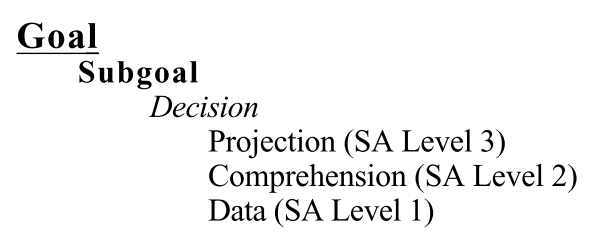
\includegraphics[width=0.7\linewidth]{figures/placeholders/SA_goal_oriented_task_analysis}
	\caption{Format of Goal-Directed Task Analysis (totaly spizgenoe name from: \cite{endsley_direct_nodate})}
	\label{fig:sagoalorientedtaskanalysis}
\end{figure}
This should yield an extensive list of questions, which assess SA information the \gls{sa} information of primary and secondary importance (for an example of the results of such analysis, see the Fig. \ref{fig:sagoalorientedtaskanalysisresultexample}).
\begin{figure}
	\centering
	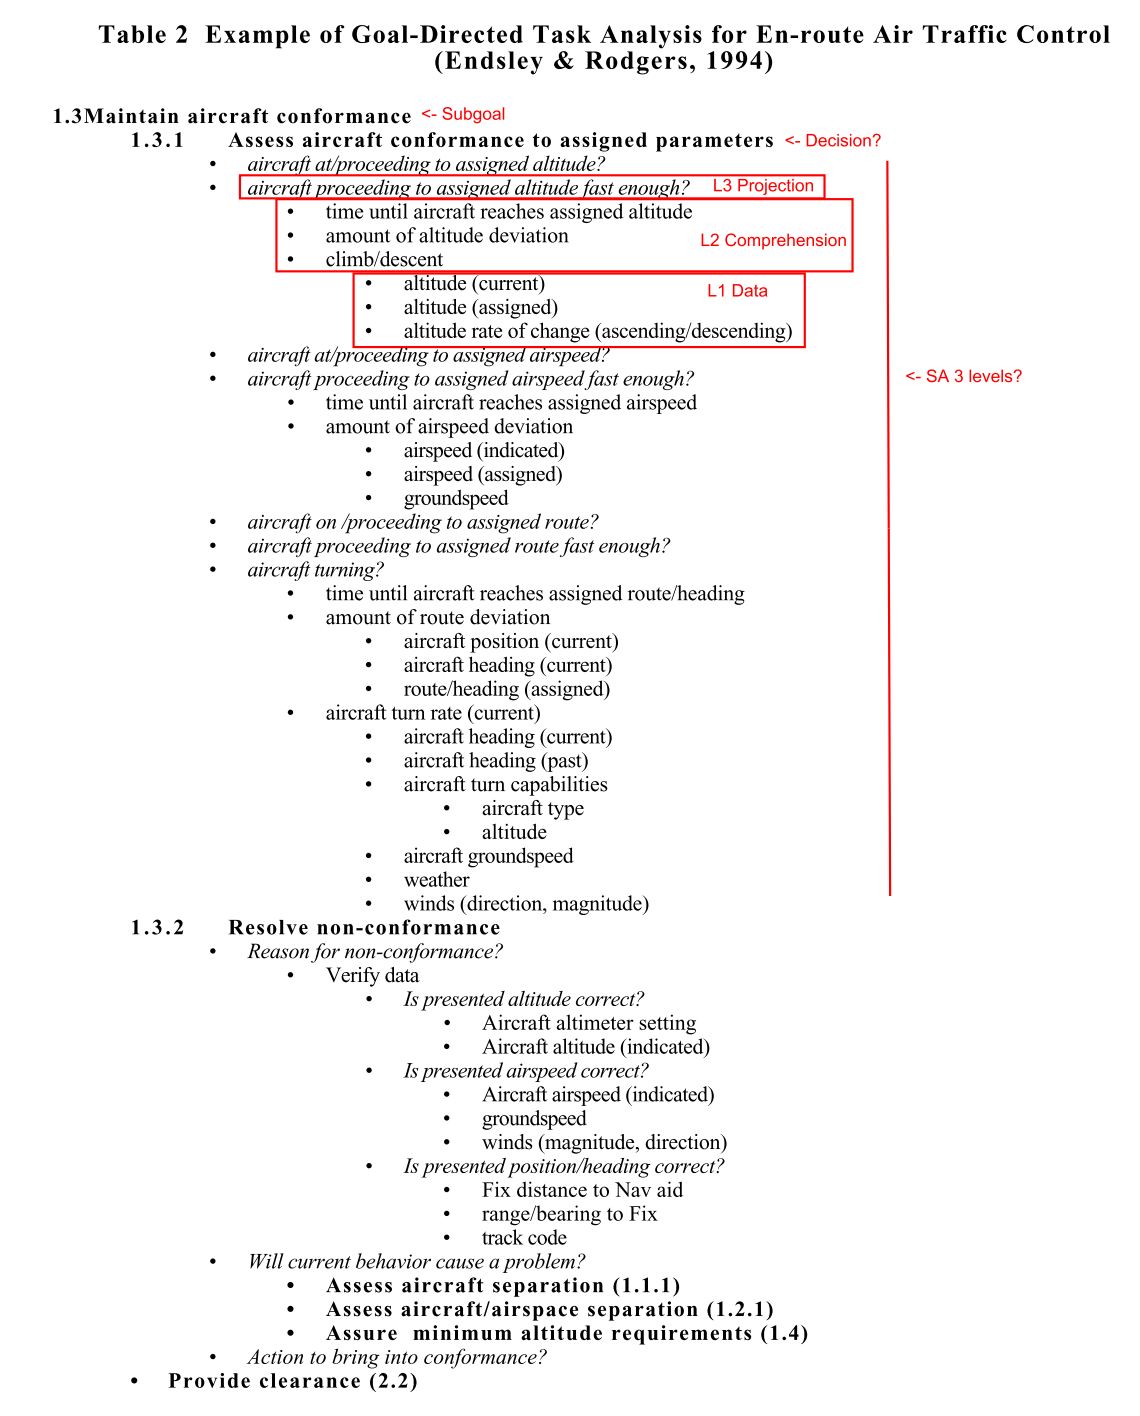
\includegraphics[width=0.7\linewidth]{figures/placeholders/SA_goal_oriented_task_analysis_result_example}
	\caption{Example of Goal-Directed Task Analysis for En-route Air Traffic Control (Endsley \& Rodgers, 1994) [from: \cite{endsley_direct_nodate}]}
	\label{fig:sagoalorientedtaskanalysisresultexample}
\end{figure}
Next, at some point in time, the simulation is halted, and the pilots are queried on the randomly selected questions from the list. When the simulation halts, all the control panels, the ?windshield of the jet-fighter, and other simulation elements are grayed-out. Not every pilot is queried on every question, the goal is to reach the desired statistical significance of the results by assessing a certain number of participants.

% This paragraph is a bit repetetive
By using this approach, it is possible to get a snapshot of the current situation in the point of view of the pilot, which is unbiased by the recall difficulties, and that can be compared to the actual situation after the experiment. Additionally, pilots' \gls{sa} is not artificially enhanced, because the questions do not always directly address the main goals in the current situation, but can concern secondary information, which is still relevant.

\cite{endsley_direct_nodate} notes that, since the introduction of \gls{sagat}, there is practical evidence that the method is valid, reliable, non-intrusive (in case of the halts are made at unpredictable time points), and is able to properly "reliably tap into memory stores" acting as a \gls{sa} index. 


o Bridge to Workspace Awareness


§ Workspace Awareness 
\gls{wa} is an extension of the idea of SA, and its adaptation to the day-to-day working scenarios. This is needed because, as authors put it: "sorting slides on a table does not seem very similar to air combat in a jet fighter", or in our case, to architectural collaboration in immersive VR environment.

o Relation to Situation awareness
o Relation to human factors’ research?
o Characteristics of awareness
* Measurement
SAGAT is sorta not applicable, because not so many elements to query upon.
o Bridge to Sonification: 
* Awareness - secondary/monitoring task \& sonification is great for monitoring -> use it for our experiment 

